\chapter{Heriyanto - 1184023}

\section{Teori}

\subsection{Definisi dan Sejarah Kecerdasan Buatan}

\subsubsection{Definisi Kecerdasan Buatan}
Kecerdasan buatan adalah sistem kecerdasan yang ditanamkan atau ditambahkan ke dalam teknologi oleh manusia, yang kemudian akan dikembangkan dalam lingkungan ilmiah atau dalam pembentukan entitas ilmiah yang ada. Kecerdasan di sini menekankan pada kemampuan memperoleh pengetahuan baru, yang dapat langsung diterapkan. Meskipun AI memiliki konotasi ilmiah, AI juga merupakan cabang dari ilmu komputer, pembelajaran, perilaku (behaviour), dan adaptasi pada mesin. \cite{purwanti2017analisis}. 

\subsubsection{Definisi Kecerdasan Buatan Menurut Para Ahli}
\begin{enumerate}
    \item Scahlkoff (1990)
    
    \par Kecerdasan Buatan merupakan bidang studi yang berusaha menerangkan dan meniru perilaku kecerdasan dalam bentuk proses komputasi.\cite{ai2011kecerdasan}
    
    \item Luger dan Stubblefield (1993)
    
    \par Kecerdasan Buatan merupakan cabang ilmu komputer yang berhubungan dengan otomatisasi perilaku yang cerdas.\cite{ai2011kecerdasan}
    
    \item Rich dan Knight (1991)
    
    \par Kecerdasan Buatan merupakan studi tentang cara membuat komputer melakukan sesuatu yang sampai saat ini, orang dapat melakukannya lebih baik.\cite{ai2011kecerdasan}
    
    \item Haag dan Keen (1996)
    
    \par Kecerdasan Buatan adalah bidang studi yang berhubungan dengan penangkapan, pemodelan, dan penyimpanan kecerdasan manusia dalam sebuah sistem teknologi sehingga sistem tersebut dapat memfasilitasi proses pengambilan keputusan yang biasanya dilakukan oleh manusia.\cite{ai2011kecerdasan}
\end{enumerate}

\subsection{Sejarah Kecerdasan Buatan}

\par Istilah kecerdasan buatan pertama kali diusulkan pada tahun 1956. Hingga saat ini, dengan peningkatan daya komputasi dan kapasitas penyimpanan, penggunaan kecerdasan buatan menjadi semakin populer. Fase penelitian awal proyek AI berlangsung sekitar tahun 1950-an, bertujuan untuk mengeksplorasi tema pemecahan masalah dan metode simbolik.

\par Pada 1960-an, Departemen Pertahanan AS juga sangat ingin mengembangkan dan melatih komputer dengan kemampuan dasar penalaran manusia. Sekitar tahun 1970-an, proyek DARPA (Defense Advanced Research Projects Agency) berhasil menyelesaikan studi kasus pemetaan jalan. Di awal abad ke-21, tepatnya tahun 2003, DARPA juga berhasil melahirkan asisten pribadi yang cerdas.

\par Setelah itu, teknologi kecerdasan buatan terus berkembang, dan hingga saat ini memasuki prosedur yang lebih detail dengan menerapkan algoritma deep learning. Di sana, kecerdasan buatan yang dikembangkan dapat melakukan tugas dan memberikan solusi yang lebih kompleks dengan kondisi yang lebih beragam.\cite{sejarahai}

\subsection{Supervised Learning dan Unsupervised Learning}

\subsubsection{Supervised Learning}

\par Supervised learning (pembelajaran terarah) adalah metode pembelajaran mesin di mana pengguna mengharapkan hasil, dan informasinya diketahui atau dimiliki oleh sistem. Artinya metode pembelajaran bekerja dengan menggunakan kembali masukan atau data pengguna dan hasil keluaran yang sebelumnya diselesaikan oleh sistem. Supervised Learning itu sendiri dapat dibagi lagi menjadi regresi dan klasifikasi.\cite{mahardhika2018analisis}

\par Regresi adalah teknik analisis yang digunakan untuk mengidentifikasi hubungan antara dua variabel atau lebih. Tujuan dari regresi adalah untuk menemukan fungsi yang memodelkan data dengan meminimalkan kesalahan atau perbedaan antara nilai prediksi dan nilai sebenarnya.

\par Klasifikasi adalah teknik yang digunakan untuk mengklasifikasikan beberapa item yang tidak berlabel ke dalam satu set kelas diskrit. Klasifikasi mencoba mempelajari hubungan antara sekumpulan variabel fitur dan variabel target. Dalam klasifikasi, variabel targetnya adalah tipe kategori.

\subsubsection{Unsupervised Learning}

\par Unsupervised Learning adalah metode lain dalam materi pembelajaran mesin, di mana tidak ada yang bisa mengetahui hasil yang diharapkan. Tujuan utama dari metode pembelajaran ini adalah agar para penggunanya dapat mengelompokkan objek-objek yang dianggap serupa pada suatu ruang atau area tertentu.\cite{unsuper}

\subsection{Data Set}

\par Kumpulan data adalah objek yang mirip dengan kamus, yang menyimpan semua data dan beberapa metadata tentang data.\cite{scikit} 

\par Saat membuat model Machine Learning, data harus dibagi menjadi satu Training Set dan satu Testing Set. Machine Learning harus diberi tahu "Data Set" mana yang akan dicapai, dan "Data Set" yang dapat digunakan untuk mencapai tujuan. "Data Set" untuk dicapai ini adalah Testing Set, dan "Data Set" untuk mencapai ini disebut Training Set.\cite{dataset}

\par Training Set adalah bagian dari Data Set yang dilatih untuk membuat prediksi atau menjalankan fungsi algoritma ML. Dengan memberikan petunjuk melalui algoritma sehingga mesin yang dilatih dapat menemukan korelasinya sendiri atau mempelajari pola dari data yang diberikan. Testing Set adalah bagian dari data set yang diuji untuk melihat akurasinya, atau dengan kata lain, untuk melihat performanya.\cite{traintest}

\section{Instalasi}

\subsection{Instalasi Scikit-Learn pada Anaconda}

\begin{enumerate}
    \item Pastikan Anaconda telah terpasang pada perangkat komputer atau laptop yang anda gunakan.
    \item Jika Anaconda belum terpasang pada perangkat anda silahkan kunjungi link berikut untuk tutorial memasang anaconda: https://docs.anaconda.com/anaconda/install/.
    \item Setelah anaconda terpasang buka command shell anaconda, dengan mengetik di start menu "Anaconda Prompt (ananconda 3)".
        \begin{figure}[H]
        \centering
        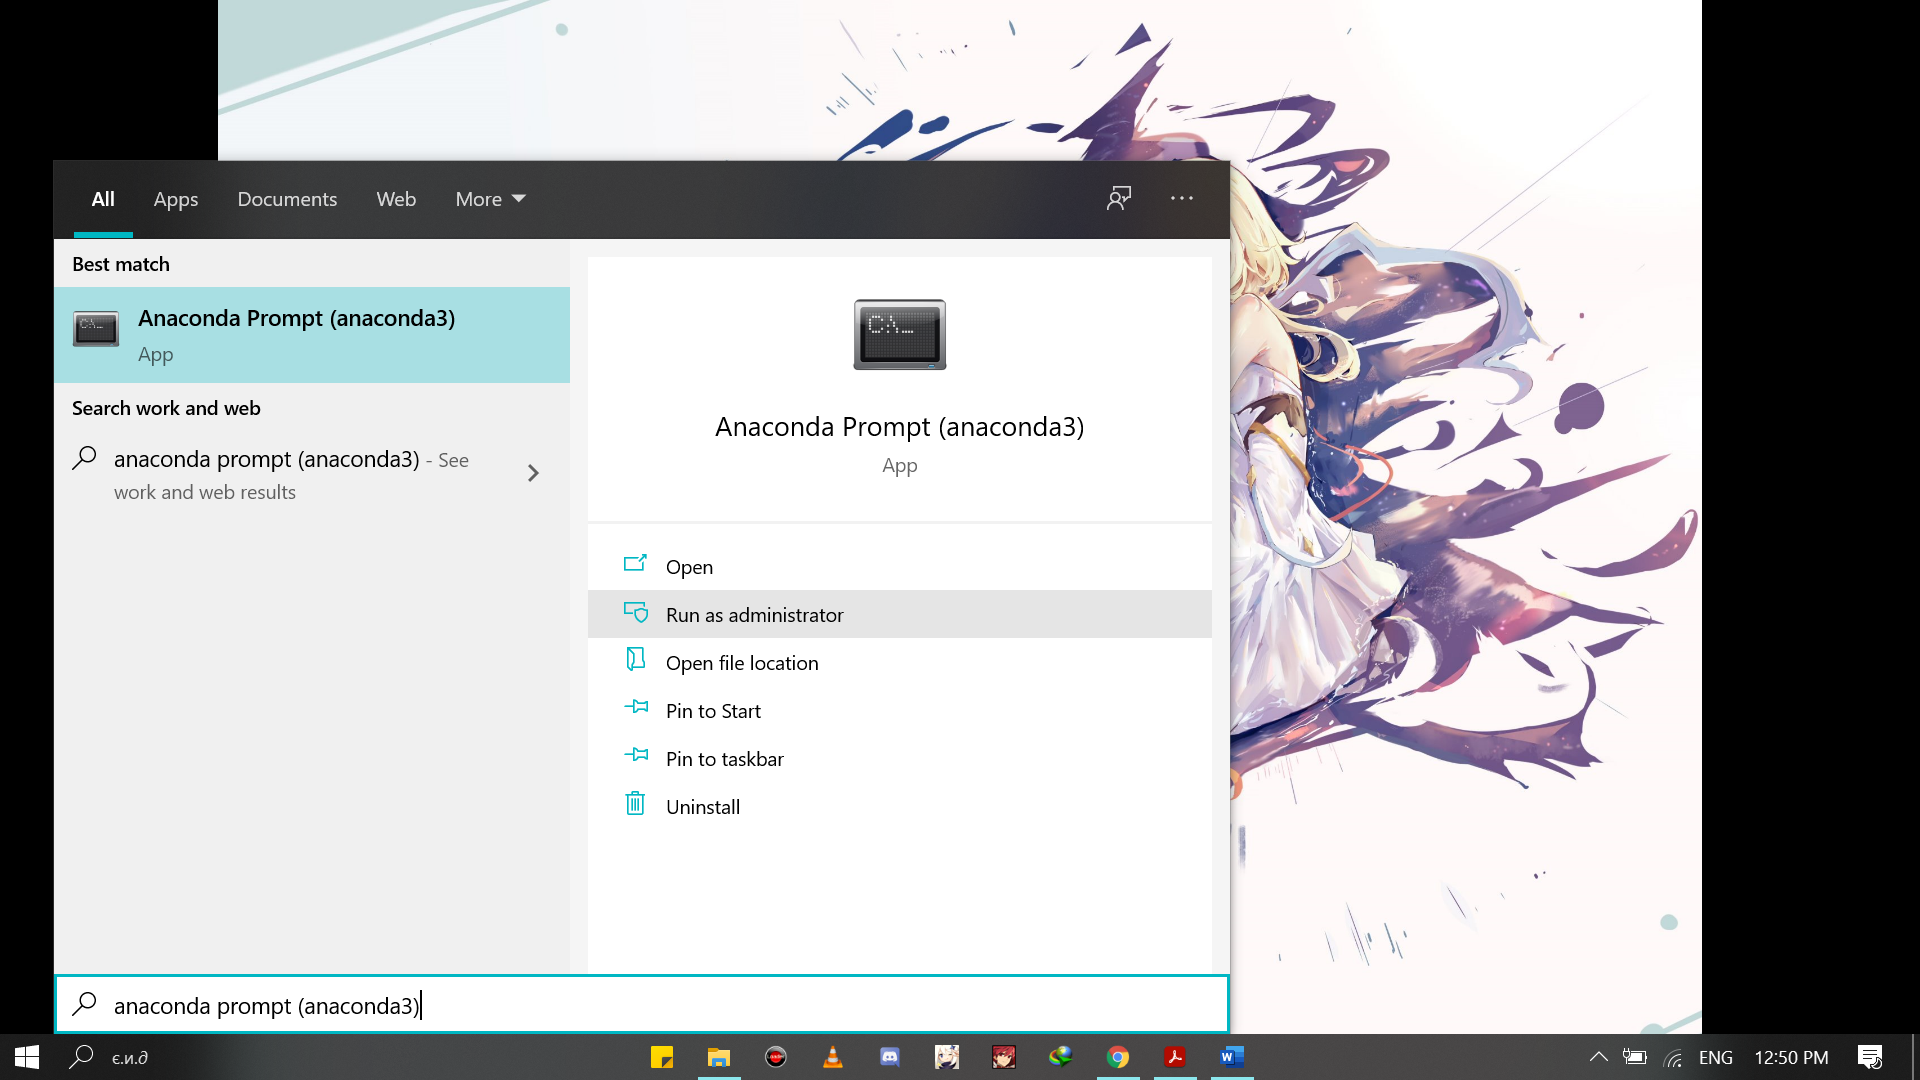
\includegraphics[width=11cm]{figures/1184023/install.png}
        \caption{Anaconda Prompt}
        \end{figure}
    \item Kemudian ketik perintah berikut untuk memasang scikit-learn library pada anaconda: conda install -c conda-forge scikit-learn, dan tunggu sampai prosesnya selesai.
        \begin{figure}[H]
        \centering
        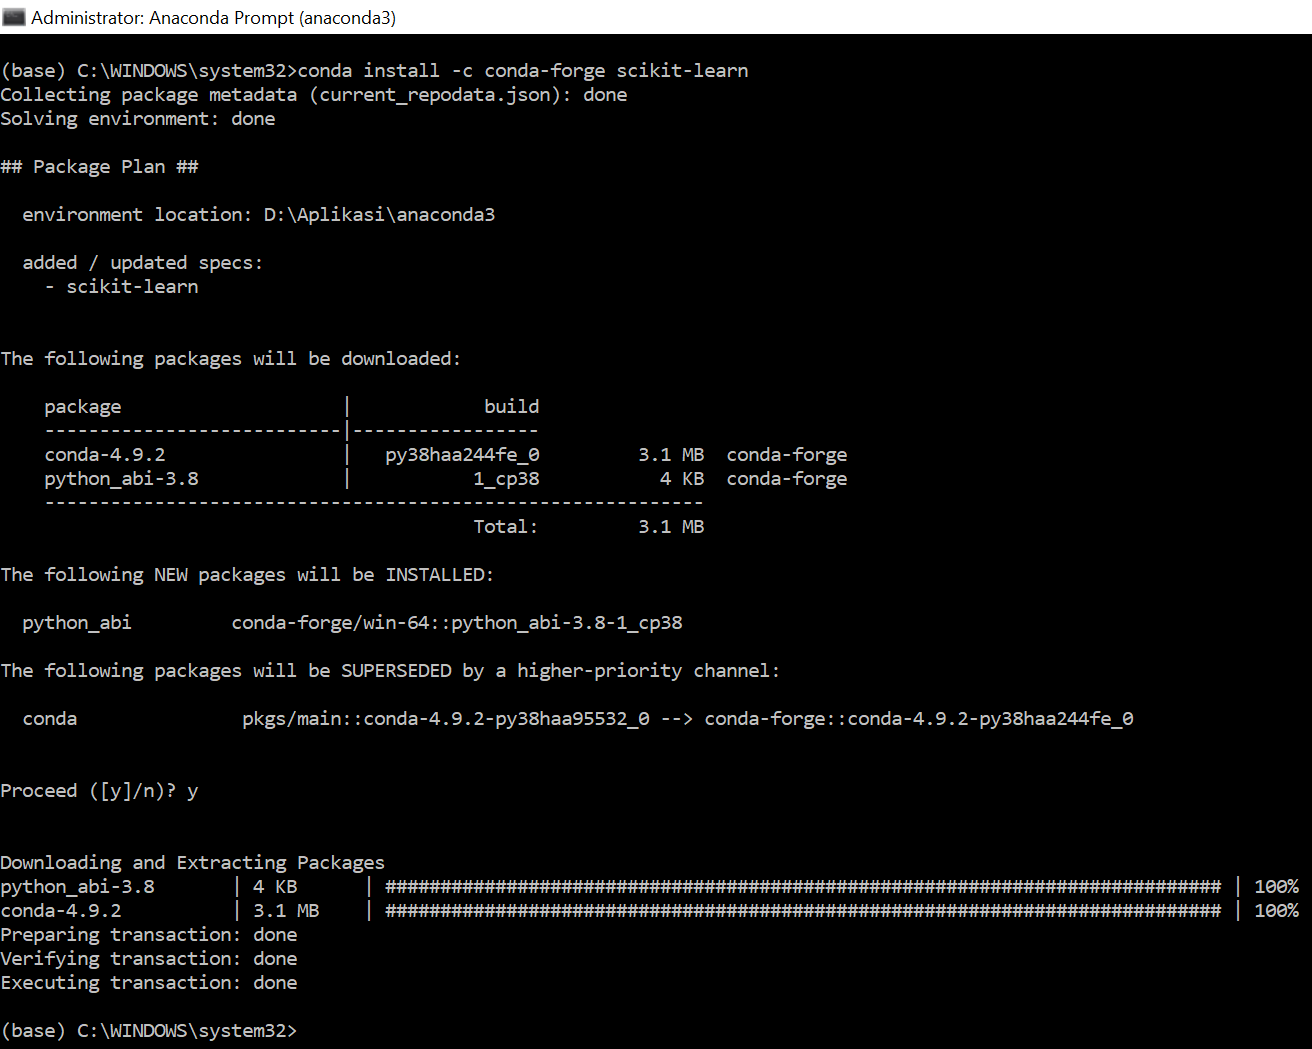
\includegraphics[width=13cm]{figures/1184023/1.PNG}
        \caption{Anaconda Prompt}
        \end{figure}
\end{enumerate}

\subsection{Loading an example dataset}

\par Scikit-learn hadir dengan beberapa dataset standar, misalnya dataset iris dan digit untuk klasifikasi dan dataset diabetes untuk regresi. Berikut ini, dimulai dengan interpreter Python menggunakan tool Spyder kemudian memuat set data iris dan digit.\cite{scikit}
    \begin{figure}[H]
    \centering
    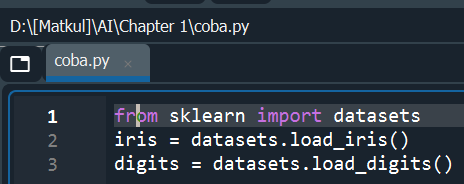
\includegraphics[width=12cm]{figures/1184023/2.PNG}
    \caption{Loading an example dataset}
    \end{figure}

\par Keterangan
    \begin{enumerate}
        \item Baris pertama: meng-import module datasets dari library sklearn.
        \item Baris kedua: iris adalah sebuah variabel dengan nilai yang memuat dataset iris dataset iris.
        \item Baris ketiga: digits adalah sebuah variabel dengan nilai yang memuat dataset digits.
    \end{enumerate}

\par Jika kode tersebut dijalankan akan menghasilkan dataset iris dan digits yang telah dimuat didalam module datasets. Berikut hasil kode yang berjalan tanpa error. Dapat dilihat pada kolom value bahwa dataset-nya telah dimuat.
    \begin{figure}[H]
    \centering
    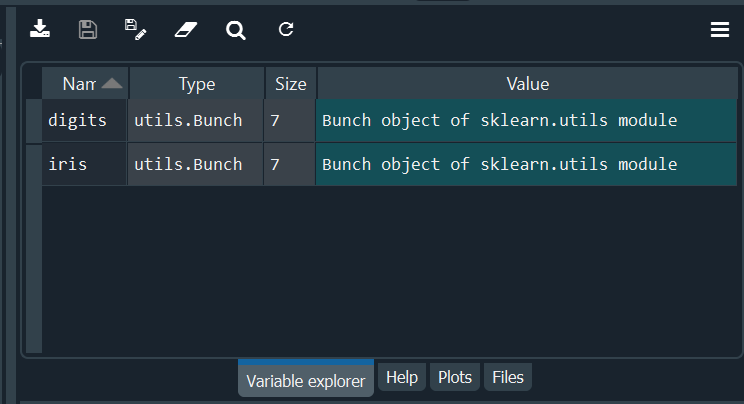
\includegraphics[width=12cm]{figures/1184023/3.PNG}
    \caption{Hasil Dataset}
    \end{figure}

\par Misalnya, untuk kumpulan data digit, Anda dapat menggunakan digits.data untuk mengakses fungsi yang dapat digunakan untuk mengklasifikasikan sampel digit:
    \begin{figure}[H]
    \centering
    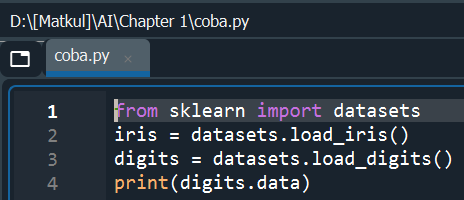
\includegraphics[width=12cm]{figures/1184023/4.PNG}
    \caption{Digits Data}
    \end{figure}

\par Disini kita menambahkan satu baris, yaitu print(digits.data) yang akan menampilkan sampel data digit. Berikut Hasilnya:
    \begin{figure}[H]
    \centering
    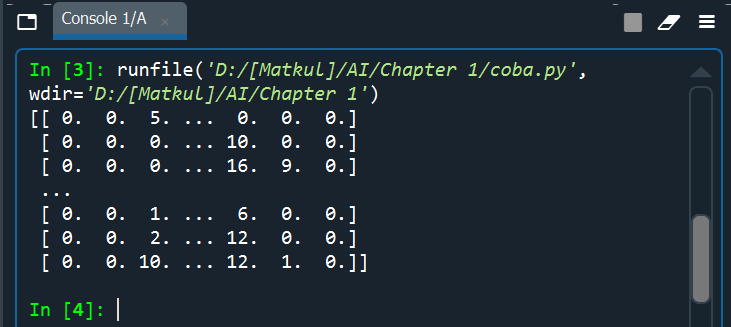
\includegraphics[width=13cm]{figures/1184023/5.PNG}
    \caption{Hasil Digits Data}
    \end{figure}
    
\par Selain digits.data, digits.target memberikan informasi dasar dari kumpulan data digit, yaitu nomor yang sesuai dengan setiap gambar digit yang ingin kita pelajari, berikut kodenya:
    \begin{figure}[H]
    \centering
    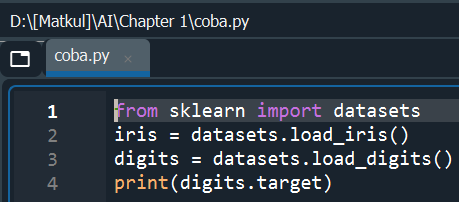
\includegraphics[width=13cm]{figures/1184023/6.PNG}
    \caption{Digits Target}
    \end{figure}

\par Seperti yang dijelaskan diatas sebelumnya digits.target akan memberikan informasi nomor setiap gambar digit yang akan dipelajari. Berikut hasilnya:
    \begin{figure}[H]
    \centering
    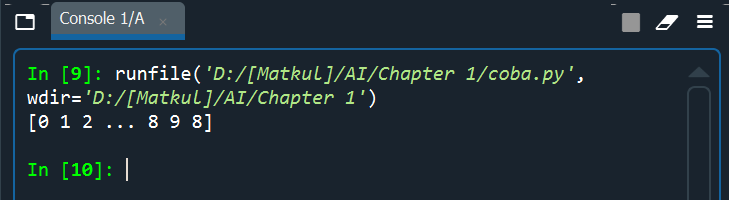
\includegraphics[width=13cm]{figures/1184023/7.PNG}
    \caption{Hasil Digits Target}
    \end{figure}

\par Meskipun data asli mungkin memiliki bentuk yang berbeda, datanya selalu berupa 2D (n-samples, n-features). Untuk digit, setiap sampel asli adalah gambar bentuk (8, 8), yang dapat diakses dengan cara berikut:
    \begin{figure}[H]
    \centering
    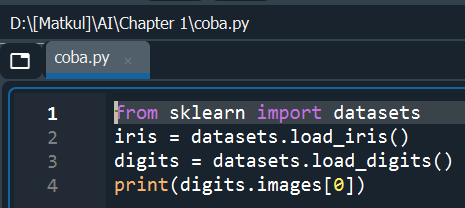
\includegraphics[width=13cm]{figures/1184023/8.PNG}
    \caption{Hasil Digits Target}
    \end{figure}

\par digits.image[0] akan menampilkan digit gambar index ke nol, yang akan menampilkan angka-angka dalam bentuk array.
    \begin{figure}[H]
    \centering
    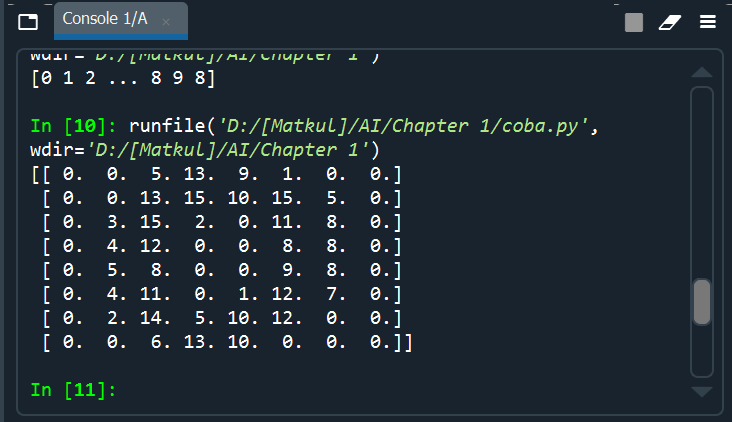
\includegraphics[width=13cm]{figures/1184023/9.PNG}
    \caption{Hasil Digits Image}
    \end{figure}

\subsection{Learning and Predicting}

\par Dalam scikit-learn, estimator yang digunakan untuk klasifikasi adalah objek Python yang mengimplementasikan metode fit (X, y) dan prediksi (T). Contoh prediktor adalah kelas sklearn.svm.SVC, yang mengimplementasikan support vector classification. Estimasi konstruktor diambil sebagai fungsi dari model parameter.

    \begin{figure}[H]
    \centering
    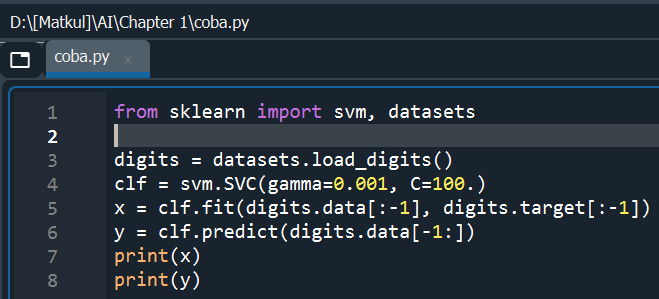
\includegraphics[width=13cm]{figures/1184023/12.PNG}
    \caption{Learning and Predicting}
    \end{figure}

\par Keterangan

    \begin{enumerate}
        \item Baris pertama mengambil module svm dan datasets dari library sklearn.
        \item Baris ketiga adalah variable dengan nama digits yang memiliki nilai untuk memuat dataset digit.
        \item Baris keempat variable clf yang memiliki value gamma=0.001 dan Classification = 100.
        \item Baris kelima variable x yang berisi clf sebagai classifier kemudian fit sebagai method yang mengambil data yang pas dari digits.data dan digits.target dengan nilai training set [:-1].
        \item Baris keenam varible y yang berisi clf sebagai classifier kemudian method predict akan memprediksi digits.data dengan nilai training set [-1:].
        \item Baris ketujuh dan kedelapan akan menampilkan hasil dari method fit dan predict.
    \end{enumerate}

\par Hasil dari method fit dan predict

    \begin{figure}[H]
    \centering
    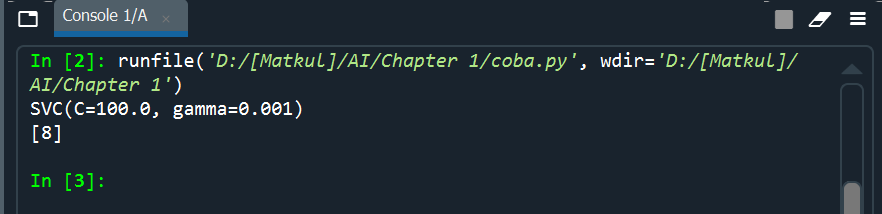
\includegraphics[width=13cm]{figures/1184023/13.PNG}
    \caption{Hasil Learning and Predicting}
    \end{figure}

\subsection{Conventions}

\subsubsection{Type Casting}

    \begin{figure}[H]
    \centering
    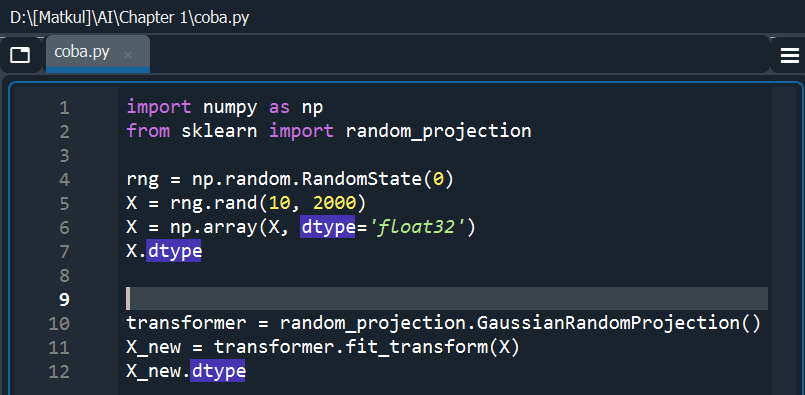
\includegraphics[width=13cm]{figures/1184023/15.PNG}
    \caption{Hasil Learning and Predicting}
    \end{figure}
    
\par Keterangan
    \begin{enumerate}
        \item Baris pertama memanggil library numpy dan dibuat dengan alias np.
        \item Baris kedua memanggil module random projection dari library sklearn.
        \item Baris keempat adalah variable rng yang mendefinisikan numpy as np, kemudian fungsi random dan attr RandomState.
        \item Baris kelima adalah variable X yang mendefinisikan variable rng, kemudian method random yang akan menentukan nilai random dari 10 - 2000.
        \item Baris keenam adalah variable X yang akan menampung nilai random sebelumnya kedalam array dengan tipe data float32.
        \item Baris ketujuh, akan mengubah tipe data nilai random float32 ke float64.
        \item Baris kesepuluh adalah sebuah variable transformer yang mendefinisikan class random projection dan memanggil fungsi GaussianRandomProjection.
        \item Baris kesebelas adalah variable X new yang akan melakukan perhitungan pada variable X.
        \item Baris keduabelas, merubah tipe data menjadi float64.
    \end{enumerate}

\par Hasil dari method X dan X new.

    \begin{figure}[H]
    \centering
    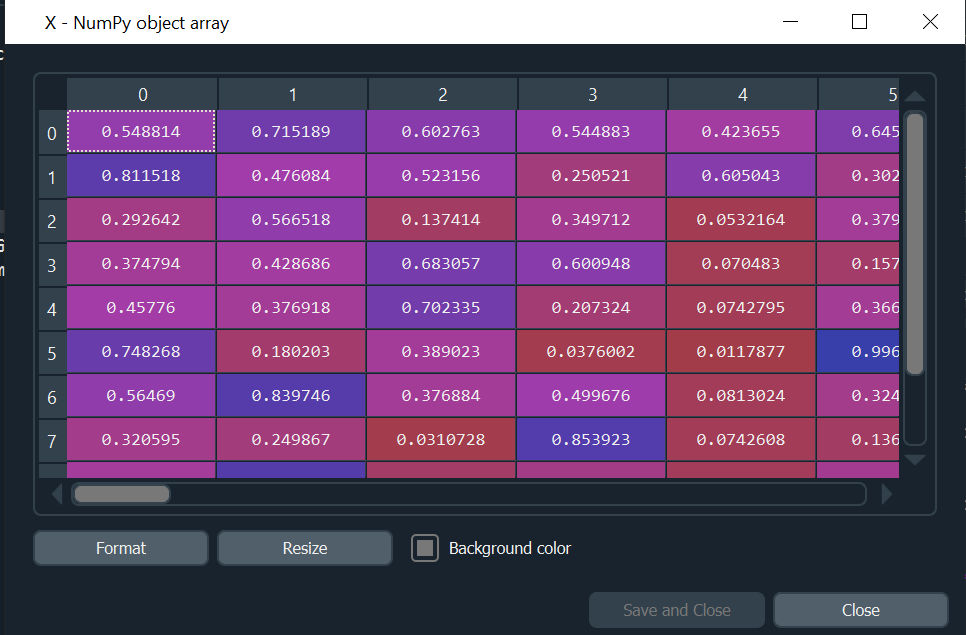
\includegraphics[width=13cm]{figures/1184023/17.PNG}
    \caption{Hasil X Numpy}
    \end{figure}
    
    \begin{figure}[H]
    \centering
    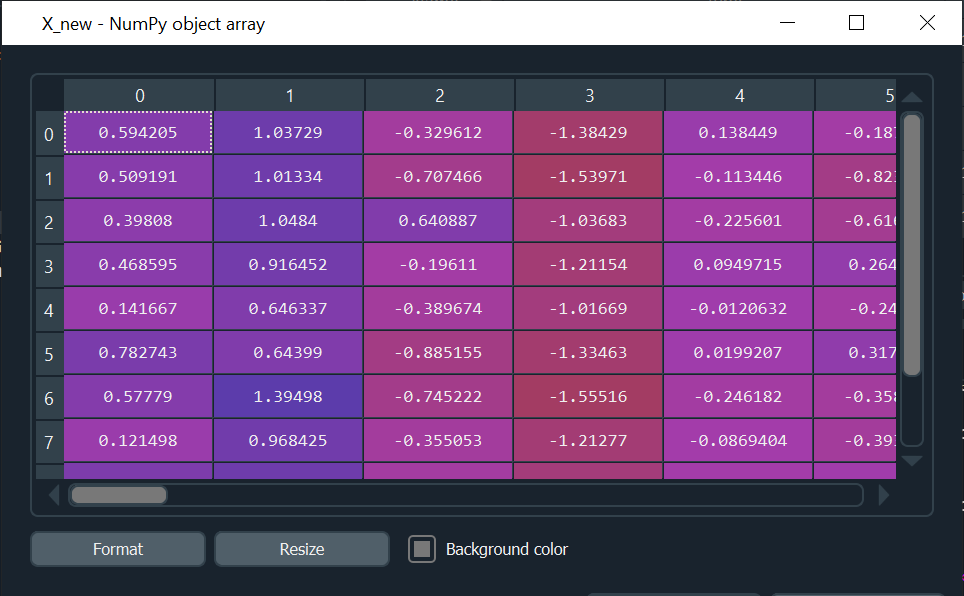
\includegraphics[width=13cm]{figures/1184023/18.PNG}
    \caption{Hasil X new Numpy}
    \end{figure}
    
\par Di sini, predict () pertama kali mengembalikan array integer, karena iris.target (array integer) digunakan dengan tepat. Prediction () kedua mengembalikan larik string karena iris.target names cocok untuk penginstalan.

    \begin{figure}[H]
    \centering
    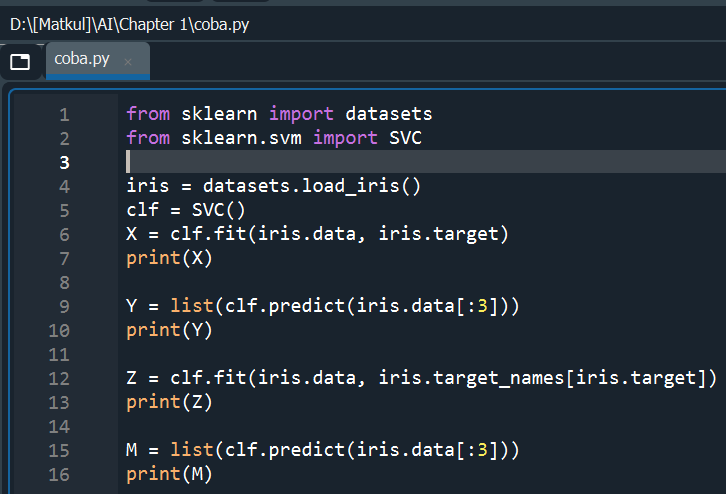
\includegraphics[width=13cm]{figures/1184023/22.PNG}
    \caption{Iris Predict}
    \end{figure}

\par Keterangan 
    \begin{enumerate}
        \item Baris pertama, memanggil module datasets dari library sklearn.
        \item Baris kedua, memanggil module SVC dari library sklearn.svm.
        \item Baris keempat, variable iris yang memuat datasets iris.
        \item Baris kelima, variable clf yang memanggil method SVC.
        \item Baris keenam, variable X yang memanggil classifier kemudian method fit yang memanggil data pas dari iris.data dan target.
        \item Baris ketujuh, menampilkan hasil variable X.
        \item Baris kesembilan, variable Y yang akan mengembalikan iris predict dalam bentuk array.
        \item Baris kesepuluh, menampilkan hasil variable Y.
        \item Baris keduabelas, memanggil classifier kemudian method fit yang memanggil data pas dari iris.names, iris.data, dan target.
        \item Baris ketigabelas, menampilkan hasil variable Z.
        \item Baris kelimabelas, variable M yang akan mengembalikan iris predict kedalam bentuk string.
        \item keenambelas, menampilkan hasil variable M.
    \end{enumerate}

\par Hasil dari iris predict.

    \begin{figure}[H]
    \centering
    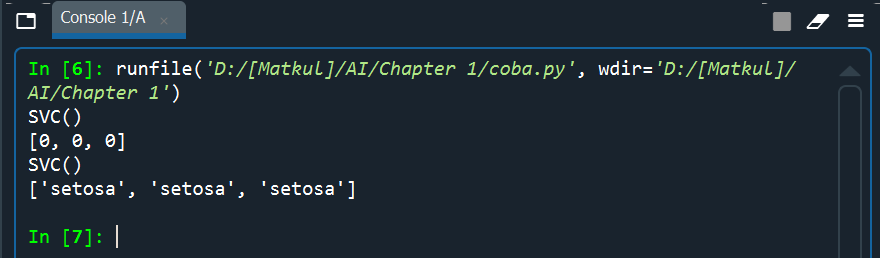
\includegraphics[width=13cm]{figures/1184023/23.PNG}
    \caption{Hasil Iris Predict}
    \end{figure}
    
\par Di sini, predict () pertama kali mengembalikan array integer, karena iris.target (array integer) digunakan dengan tepat. Prediction () kedua mengembalikan string karena iris.targetnames cocok untuk penginstalan.

\subsubsection{Refitting and updating parameters}

\par Hyperparameter dari estimator dapat diperbarui setelah dibuat dengan metode setparams (). Memanggil fit () beberapa kali akan menimpa fit () yang dipelajari sebelumnya:

    \begin{figure}[H]
    \centering
    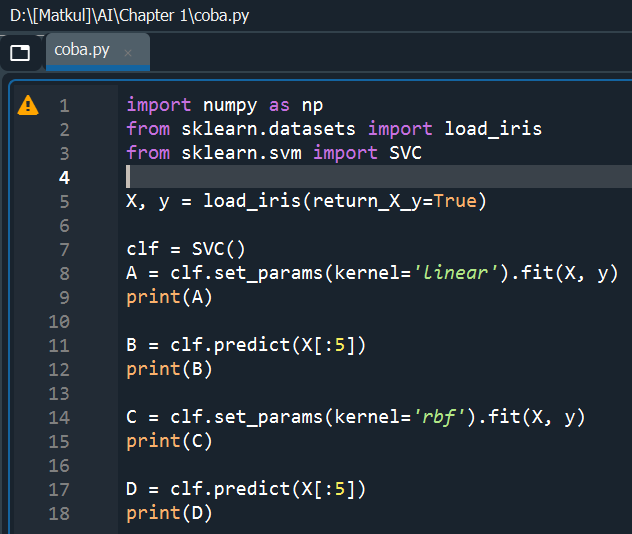
\includegraphics[width=13cm]{figures/1184023/24.PNG}
    \caption{Refitting and updating parameters}
    \end{figure}

\par Keterangan:
    \begin{enumerate}
        \item Baris pertama, memanggil library numpy dengan alias np.
        \item Baris kedua, memanggil module load iris dari library sklearn.datasets.
        \item Baris ketiga, memanggil module SVC dari library sklearn.svm.
        \item Baris kelima, mengisi variable X dan y dengan datasets iris.
        \item Baris ketujuh, mendifinisikan clf sebagai fungsi SVC.
        \item Baris kedelapan, mengubah rbf menjadi linear melalui SVC.setparams kedalam variable A.
        \item Baris kesembilan, menampilkan hasil variable A.
        \item Baris kesebelas, clf dengan method predict akan menampilkan data X dalam array sebanyak 5 data kedalam variable B.
        \item Baris keduabelas, menampilkan hasil variable B.
        \item Baris keempatbelas, mengubah linear ke rbf melalui SVC.setparams kedalam variable C.
        \item Baris kelimabelas, menampilkan hasil variable C.
        \item Baris ketujuhbelas, clf dengan method predict akan menampilkan data X dalam array sebanyak 5 data kedalam variable D.
        \item Baris kedelapanbelas, menampilkan hasil variable D.
    \end{enumerate}

\par Hasil dari Refitting and updating parameters.

    \begin{figure}[H]
    \centering
    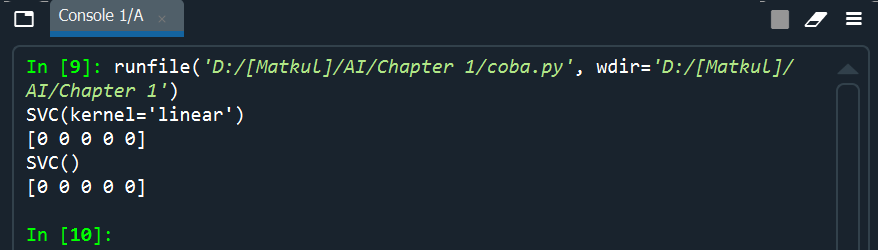
\includegraphics[width=13cm]{figures/1184023/25.PNG}
    \caption{Hasil Refitting and updating parameters}
    \end{figure}

\par Di sini, kernel default rbf pertama-tama diubah menjadi linier oleh SVC.setparams () setelah membuat estimator, dan kemudian diubah kembali ke rbf untuk mereparasi estimator dan membuat prediksi kedua.

\subsubsection{Multiclass vs. multilabel fitting}

\par Saat menggunakan multiclass classifiers, tugas learning and prediction yang dilakukan bergantung pada format data target yang sesuai, yang bergantung pada:

    \begin{figure}[H]
    \centering
    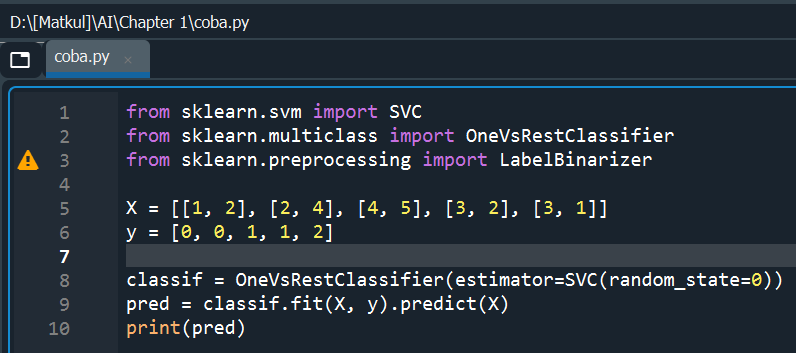
\includegraphics[width=13cm]{figures/1184023/26.PNG}
    \caption{Multiclass Predict}
    \end{figure}

\par Keterangan:
    \begin{enumerate}
        \item Baris pertama, memanggil module SVC dari library sklearn.svm.
        \item Baris kedua, memanggil module OneVsRestClassifier dari library sklearn.multiclass.
        \item Baris ketiga, memanggil module LabelBinarizer dari library sklearn.preprocessing.
        \item Baris kelima dan keenam, variable x dan y yang berisi data array.
        \item Baris kedelapan, menggunakan method OneVsRestClassifier dengan fungsi SVC sebagai estimator untuk menghasilkan data random yang didefiniskan kedalam classif.
        \item Baris kesembilan, memberikan hasil multiclass prediksi yang sesuai kedalam variable pred.
        \item Baris kesepuluh, menampilkan hasil variable pred.
    \end{enumerate}

\par Hasil dari Multiclass Predict.

    \begin{figure}[H]
    \centering
    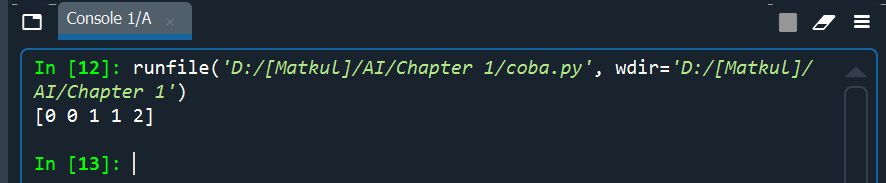
\includegraphics[width=13cm]{figures/1184023/27.PNG}
    \caption{Hasil Multiclass Predict}
    \end{figure}

\par Dalam kasus di atas, classifier cocok untuk pred label multiclass, sehingga metode predict () menyediakan prediksi multiclass yang sesuai. Dimungkinkan juga untuk menyesuaikan dengan array 2d indikator label biner:

    \begin{figure}[H]
    \centering
    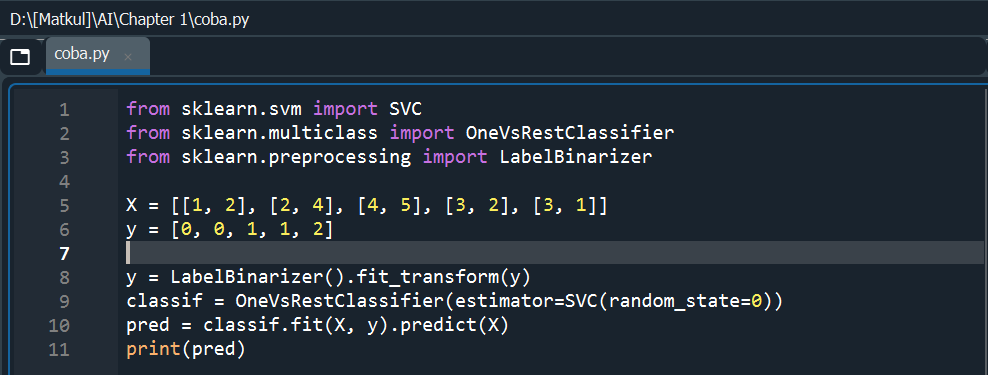
\includegraphics[width=13cm]{figures/1184023/28.PNG}
    \caption{Multiclass Predict 2}
    \end{figure}
    
\par Keterangan:
    \begin{enumerate}
        \item Baris pertama, memanggil module SVC dari library sklearn.svm.
        \item Baris kedua, memanggil module OneVsRestClassifier dari library sklearn.multiclass.
        \item Baris ketiga, memanggil module LabelBinarizer dari library sklearn.preprocessing.
        \item Baris kelima dan keenam, variable x dan y yang berisi data array.
        \item Baris kedelapan, classifier fit() merepresentasi variable y dengan LabelBinarizer.
        \item Baris kesembilan, menggunakan method OneVsRestClassifier dengan fungsi SVC sebagai estimator untuk menghasilkan data random yang didefiniskan kedalam classif.
        \item Baris kesepuluh, memberikan hasil multiclass prediksi yang sesuai kedalam variable pred.
        \item Baris kesebelas, menampilkan hasil variable pred. 
    \end{enumerate}

\par Hasil dari Multiclass Predict 2

    \begin{figure}[H]
    \centering
    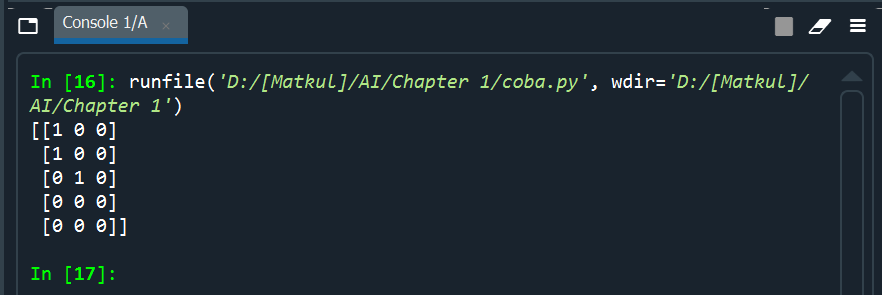
\includegraphics[width=13cm]{figures/1184023/29.PNG}
    \caption{Hasil Multiclass Predict 2}
    \end{figure}

\par Di sini, LabelBinarizer digunakan untuk menyesuaikan pengklasifikasi dengan representasi label biner pred dari y. Dalam kasus ini, predict () mengembalikan pred dalam bentuk array yang mewakili prediksi yang sesuai.

\par MultiLabel Fitting, dalam kasus ini, beberapa label ditetapkan ke classifier yang sesuai untuk setiap sampel. MultiLabelBinarizer digunakan untuk membuat binarisasi pred multilabel agar sesuai. Akibatnya, predict () mengembalikan larik pred yang berisi beberapa label yang diprediksi untuk setiap instance.

    \begin{figure}[H]
    \centering
    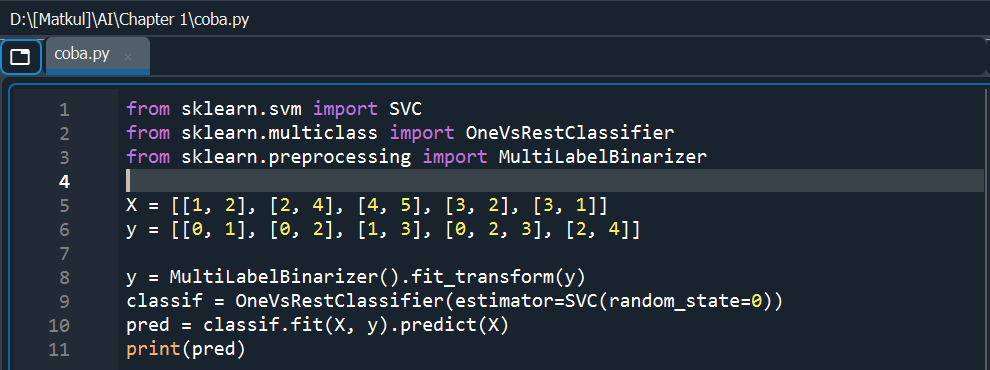
\includegraphics[width=13cm]{figures/1184023/30.PNG}
    \caption{MultiLabel Fitting}
    \end{figure}

\par Keterangan:
    \begin{enumerate}
        \item Baris pertama, memanggil module SVC dari library sklearn.svm.
        \item Baris kedua, memanggil module OneVsRestClassifier dari library sklearn.multiclass.
        \item Baris ketiga, memanggil module LabelBinarizer dari library sklearn.preprocessing.
        \item Baris kelima dan keenam, variable x dan y yang berisi data array.
        \item Baris kedelapan, classifier fit() merepresentasi variable y dengan MultiLabelBinarizer.
        \item Baris kesembilan, menggunakan method OneVsRestClassifier dengan fungsi SVC sebagai estimator untuk menghasilkan data random yang didefiniskan kedalam classif.
        \item Baris kesepuluh, memberikan hasil multiclass prediksi yang sesuai kedalam variable pred.
        \item Baris kesebelas, menampilkan hasil variable pred. 
    \end{enumerate}

\par Hasil dari Multilabel Fitting

    \begin{figure}[H]
    \centering
    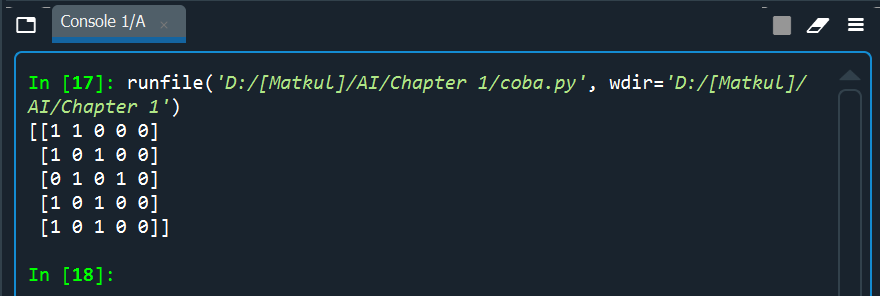
\includegraphics[width=13cm]{figures/1184023/31.PNG}
    \caption{Hasil MultiLabel Fitting}
    \end{figure}

\section{Penanganan Error}

\subsection{Error 1}

    \begin{figure}[H]
    \centering
    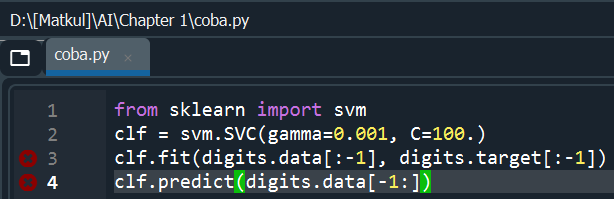
\includegraphics[width=13cm]{figures/1184023/error/1.PNG}
    \caption{Hasil MultiLabel Fitting}
    \end{figure}

\par Pada baris tiga dan empat terdapat error, yaitu sebagai berikut:

    \begin{figure}[H]
    \centering
    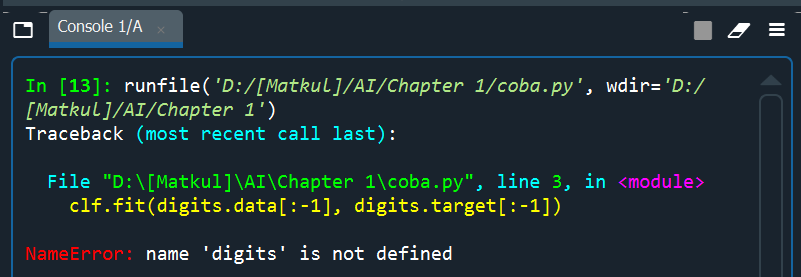
\includegraphics[width=13cm]{figures/1184023/error/2.PNG}
    \caption{Hasil MultiLabel Fitting}
    \end{figure}

\par Nama errornya adalah karena "digits" tidak terdifinisikan. Untuk penanganannya kita harus mendefinisikan digits sebagai berikut:

    \begin{figure}[H]
    \centering
    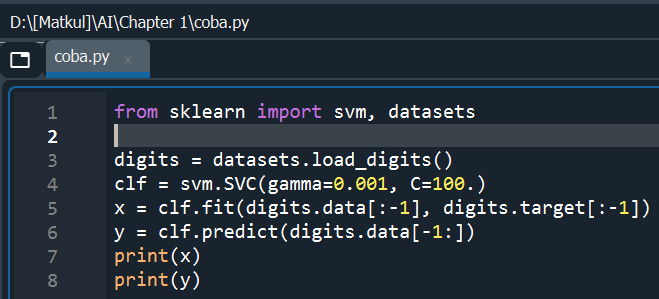
\includegraphics[width=13cm]{figures/1184023/12.PNG}
    \caption{Learning and Predicting}
    \end{figure}

\par Dapat dilihat perbedaannya pada baris pertama dan ketiga, pada baris pertama, memanggil modul datasets yang sebelumnya tidak ada dan kemudian pada baris ketiga, digits didefinisikan.